\subsection*{Модель Калдора-Калецкого}
\addcontentsline{toc}{subsection}{Модель Калдора-Калецкого}

\textbf{Задание:}\\
Провести численный анализ и качественный анализ модели Калдора-Калецкого в среде AnyLogic.\\

\textbf{Решение:}\\
$Y$ -- основной доход\\
$K$ -- основной капитал\\
$I$ -- инвестиции\\
$\alpha$ -- коэффициент пропорциональности инвестиций и сбережений\\
$\delta$ -- степень обесценивания капитала\\
$\beta$ -- степень влияния капитала на инвестиции\\
$\tau_1, \tau_2$ -- величины задержки капитала и инвестиций соответственно

\begin{align*}
	\begin{cases}
		\dfrac{dY}{dt} = \alpha I (Y(t + \tau_1)) + \alpha \beta K (t + \tau_2) - \alpha \gamma Y(t)\\[10pt]
		\dfrac{dK}{dt} = I(Y(t)) + (\beta - \delta) K(t)
	\end{cases}
\end{align*}

Сформулированная система Калдора-Калецкого включает функциональное дифференциально-разностное уравнение с запаздыванием. Это такой тип дифференциальных уравнений, в котором текущее поведение системы зависит от прошлой истории. Инвестиции зависят от дохода в момент принятия инвестиционные решения, и капитала в момент внедрения инвестиций. Последнее вытекает из того обстоятельства, что в момент времени $t$ могут существовать инвестиции, которые будут внедряться в экономику во временном интервале между $t-\tau$ и $t$. Таким образом, комбинированная модель Калдора-Калецкого позволяет, при планировании новых инвестиций, учесть полученный в этом интервале капитал.\\

В результате бифуркационного анализа было выявлено, что при $\tau_1 = \tau_2 = 0$ состояние равновесия -- неустойчивый фокус, при $\tau_1 > 0, \tau_2 = 0$ состояние равновесия -- устойчивый фокус, при $\tau_1 > 0, \tau_2 < 0, \tau_1 = \tau_2$ состояние равновесия -- устойчивый фокус, $\tau_1 = 0, \tau_2 > 0$ состояние равновесия -- неустойчивый фокус, при $\tau_1 > 0, \tau_2 > 0, \tau_1 > \tau_2$ состояние равновесия -- устойчивый фокус, при $\tau_1 > 0, \tau_2 > 0, \tau_1 < \tau_2$ состояние равновесия -- неустойчивый фокус.\\

\newpage

В соответствии с рассмотренными случаями, данная модель была реализована в среде моделирования AnyLogic с различными параметрами. (Рисунок \ref{fig:kaldor1})
\begin{figure}[h]
	\centering 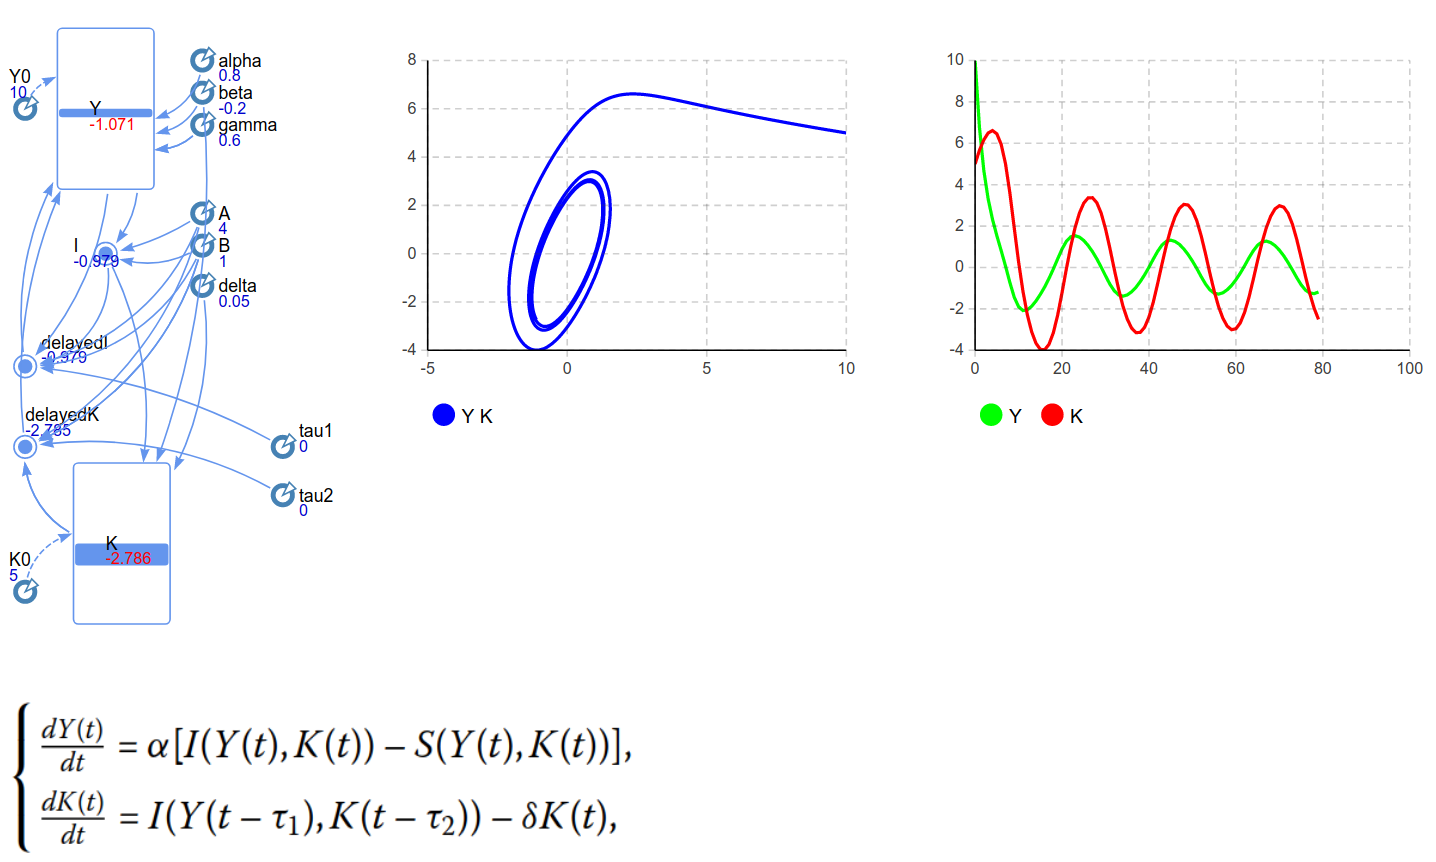
\includegraphics[scale=0.25]{kaldor1}
	\caption{Результаты построения модели Калдора-Калецкого в AnyLogic с параметрами: $\tau_1 = \tau_2 = 0$}
	\label{fig:kaldor1}
\end{figure}

\begin{figure}[h]
	\centering 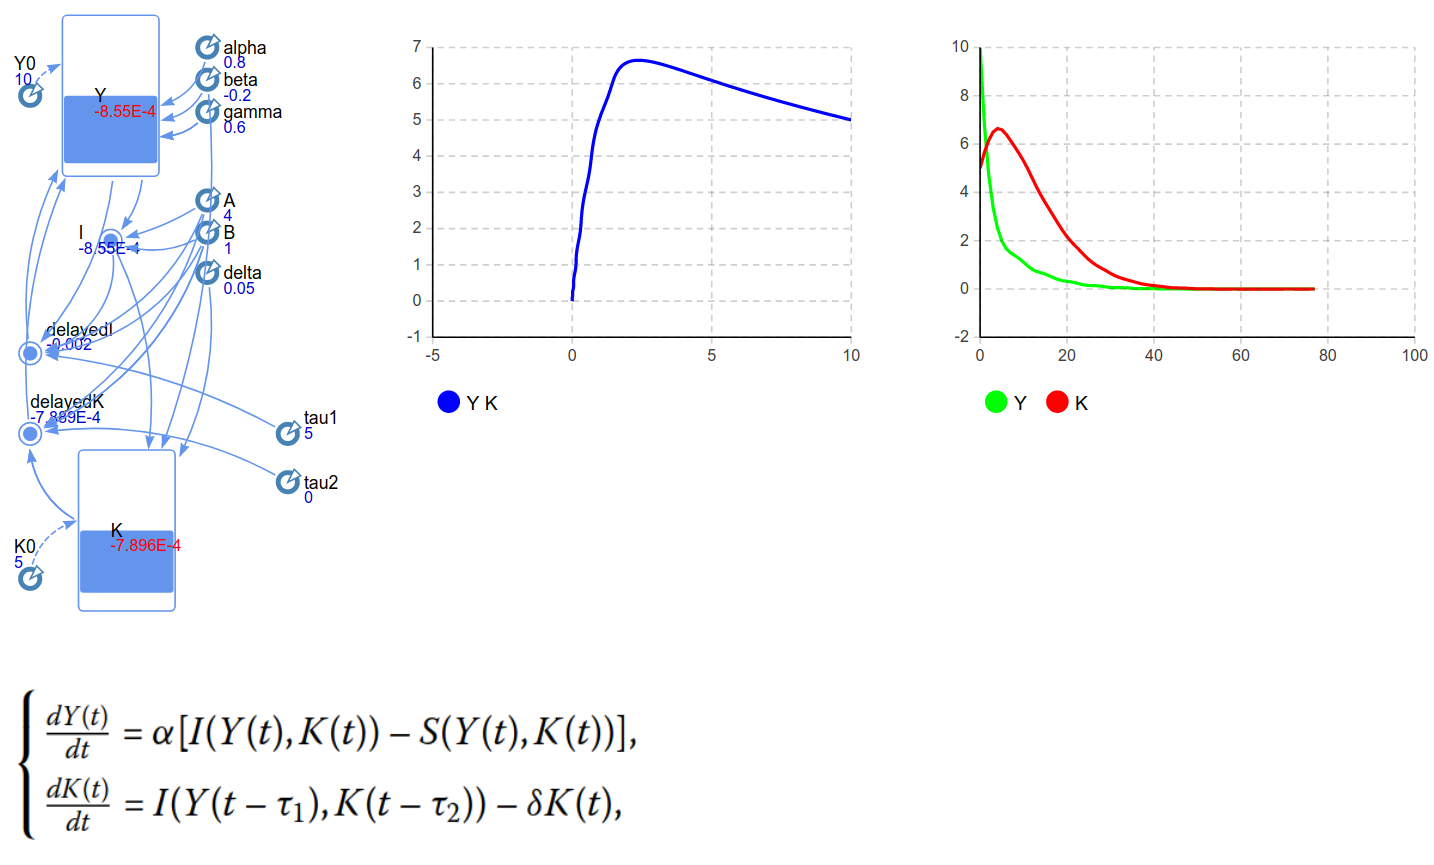
\includegraphics[scale=0.2]{kaldor2}
	\caption{Результаты построения модели Калдора-Калецкого в AnyLogic с параметрами: $\tau_1 > 0, \tau_2 = 0$}
	\label{fig:kaldor2}
\end{figure}

\newpage

\begin{figure}[h]
	\centering 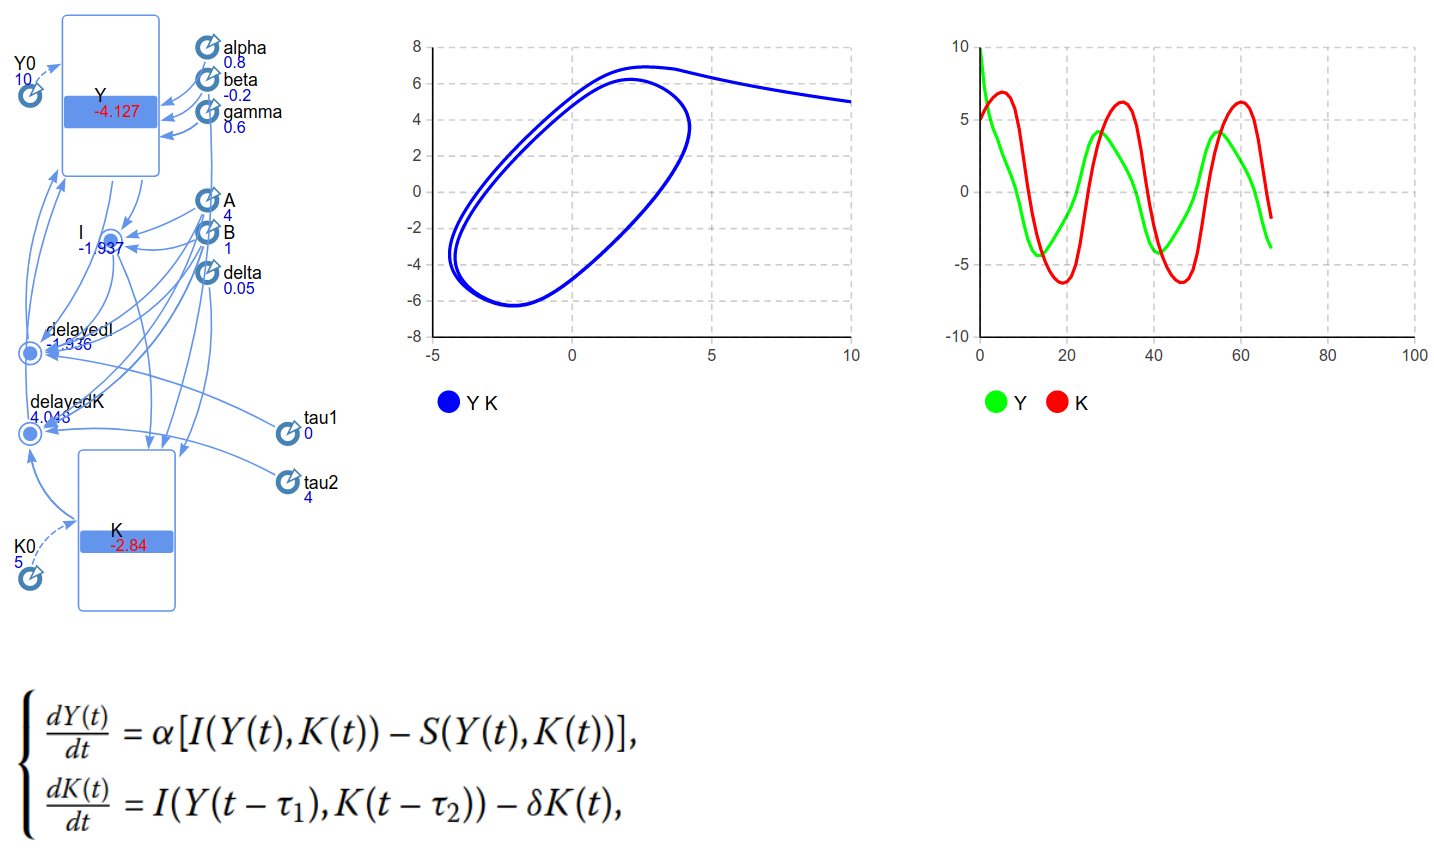
\includegraphics[scale=0.25]{kaldor3}
	\caption{Результаты построения модели Калдора-Калецкого в AnyLogic с параметрами: $\tau_1 = 0, \tau_2 > 0$}
	\label{fig:kaldor3}
\end{figure}

\begin{figure}[h]
	\centering 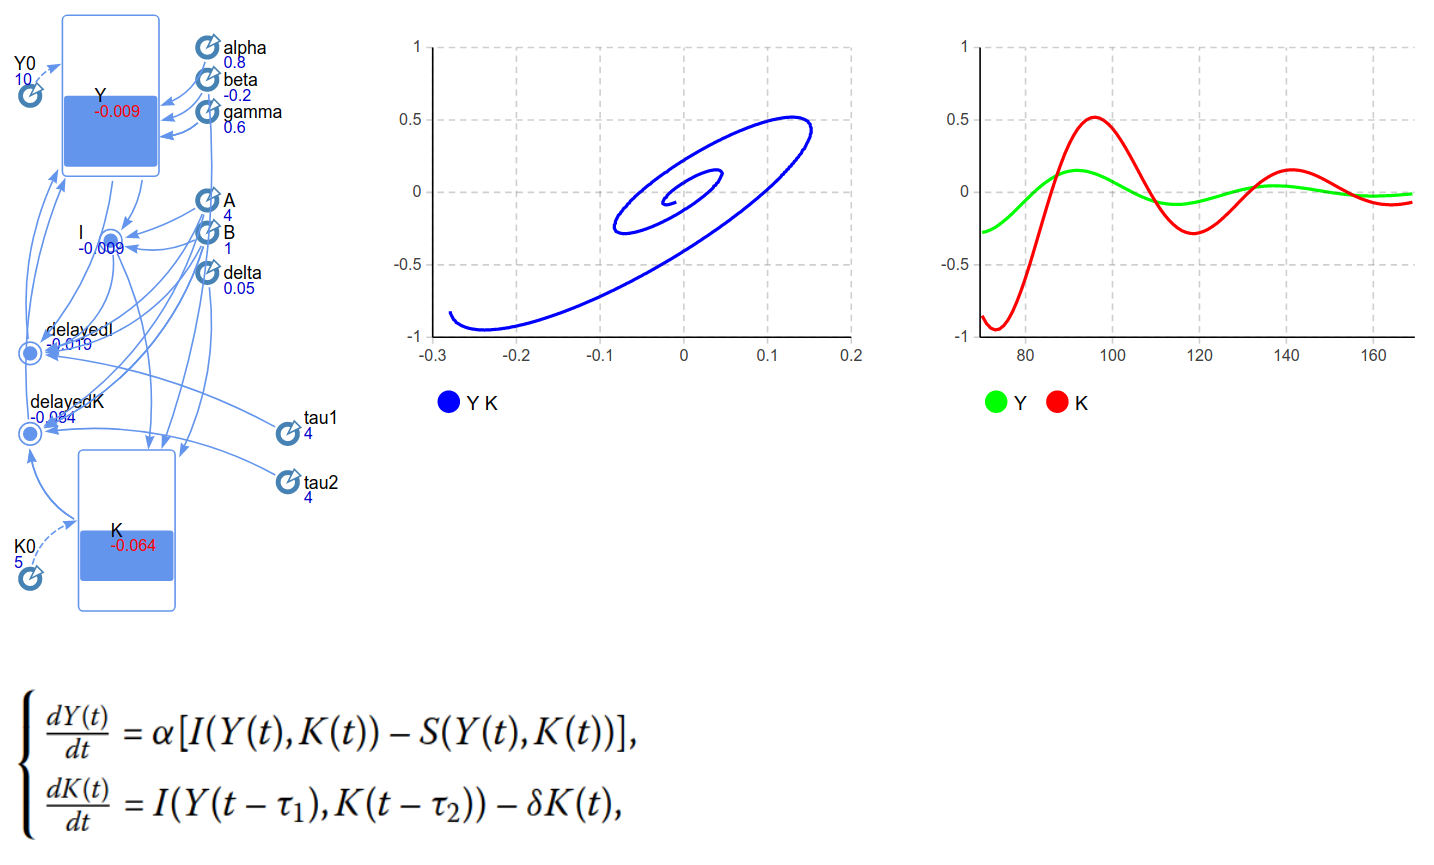
\includegraphics[scale=0.22]{kaldor4}
	\caption{Результаты построения модели Калдора-Калецкого в AnyLogic с параметрами: $\tau_1 > 0, \tau_2 > 0, \tau_1 = \tau_2$}
	\label{fig:kaldor4}
\end{figure}

\newpage

\begin{figure}[h]
	\centering 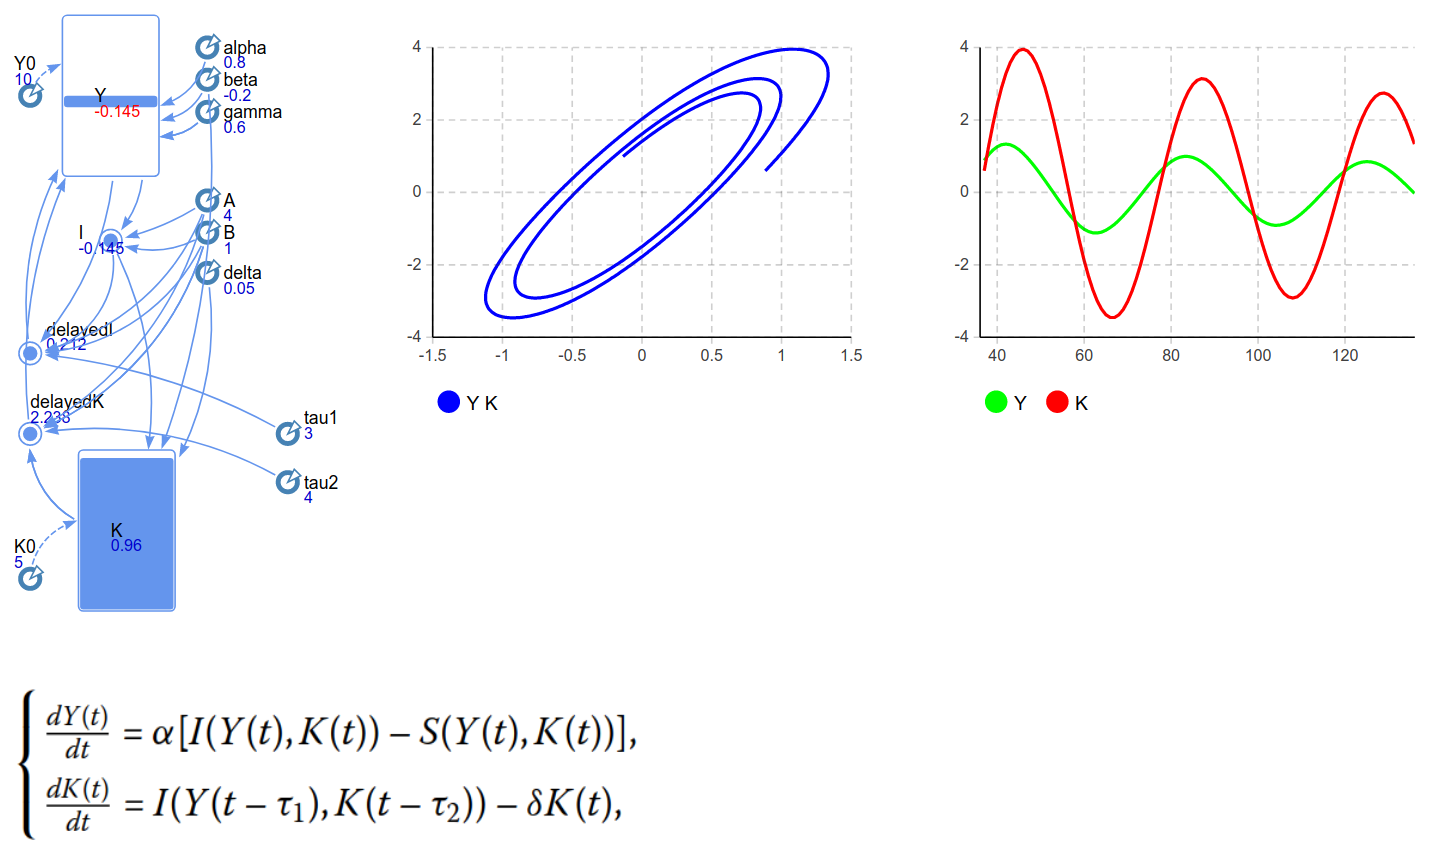
\includegraphics[scale=0.25]{kaldor5}
	\caption{Результаты построения модели Калдора-Калецкого в AnyLogic с параметрами: $\tau_1 > 0, \tau_2 > 0, \tau_1 < \tau_2$}
	\label{fig:kaldor5}
\end{figure}

Таким образом, был проведен численный и качественный анализ модели Калдора-Калецкого, а так же были найдены соотношения параметров, при которых происходит бифуркация.